\documentclass[aspectratio=169, 11pt]{beamer}
\usetheme[progressbar=frametitle, numbering=fraction]{metropolis}
\usepackage[T5]{fontenc}
\usepackage[utf8]{inputenc}
\usepackage[vietnamese]{babel}
\usepackage{lmodern}
\usepackage{booktabs, array, colortbl}
\usepackage{tikz}
\usetikzlibrary{arrows.meta,positioning,fit,backgrounds,shapes.geometric}
\graphicspath{{../writing/figures/}}

\definecolor{haitayblue}{RGB}{31,78,121}
\definecolor{haitayorange}{RGB}{235,104,52}
\definecolor{haitaygreen}{RGB}{46,125,50}
\setbeamercolor{frametitle}{bg=haitayblue}
\setbeamercolor{progress bar}{fg=haitayorange}
\setbeamercolor{alerted text}{fg=haitayorange}
\newcolumntype{L}[1]{>{\raggedright\arraybackslash}p{#1}}
\newcolumntype{R}[1]{>{\raggedleft\arraybackslash}p{#1}}
\newcolumntype{C}[1]{>{\centering\arraybackslash}p{#1}}
\newcommand{\hrow}{\rowcolor{haitayblue}}
\newcommand{\srow}{\rowcolor{haitayblue!8}}
\newcommand{\hc}[1]{\textcolor{white}{\textbf{#1}}}
% Metropolis sizes the title minipage to \paperheight, which overflows the
% plain frame by about 16pt; the same template one line shorter fits.
\makeatletter
\setbeamertemplate{title page}{
  \begin{minipage}[b][\dimexpr\paperheight-18pt\relax]{\textwidth}
    \vfill%
    \usebeamertemplate*{title}
    \usebeamertemplate*{subtitle}
    \usebeamertemplate*{title separator}
    \usebeamertemplate*{author}
    \usebeamertemplate*{date}
    \usebeamertemplate*{institute}
    \vfill
    \vspace*{1mm}
  \end{minipage}
}
\makeatother
% Item the team must still supply before or during the presentation.
\newcommand{\cbs}[1]{\textcolor{red!75!black}{\textbf{[#1]}}}

\title{Haitay}
\subtitle{Thiết bị bấm giờ speedcubing, Project Checkpoint 1}
\author{Nhóm Hai Người}
\institute{IT4735 IoT và Ứng dụng, lớp 175680, GV: TS. Đặng Tuấn Linh}
\date{13/11/2026}

\begin{document}
\maketitle

% ================================================================ 1
\begin{frame}{1. Giới thiệu dự án}
\begin{columns}[T]
\column{0.54\textwidth}
\textbf{Haitay}: bộ bấm giờ hai pad kiểu Stackmat. Thiết bị tự lưu mọi lượt solve, tính Ao5, Ao12, Ao100, rồi đồng bộ qua Bluetooth LE sang máy tính.

\medskip
\small
\begin{tabular}{L{3.2cm} L{1.9cm}}
\toprule
\hrow \hc{Nhóm Hai Người} & \hc{MSSV} \\
\midrule
\srow Phạm Gia Hưng & 20230036 \\
Đỗ Trường Giang & 20235066 \\
\srow Dương Thanh Minh & 20230047 \\
Nguyễn Anh Bảo & 20220014 \\
\bottomrule
\end{tabular}
\column{0.43\textwidth}
\centering
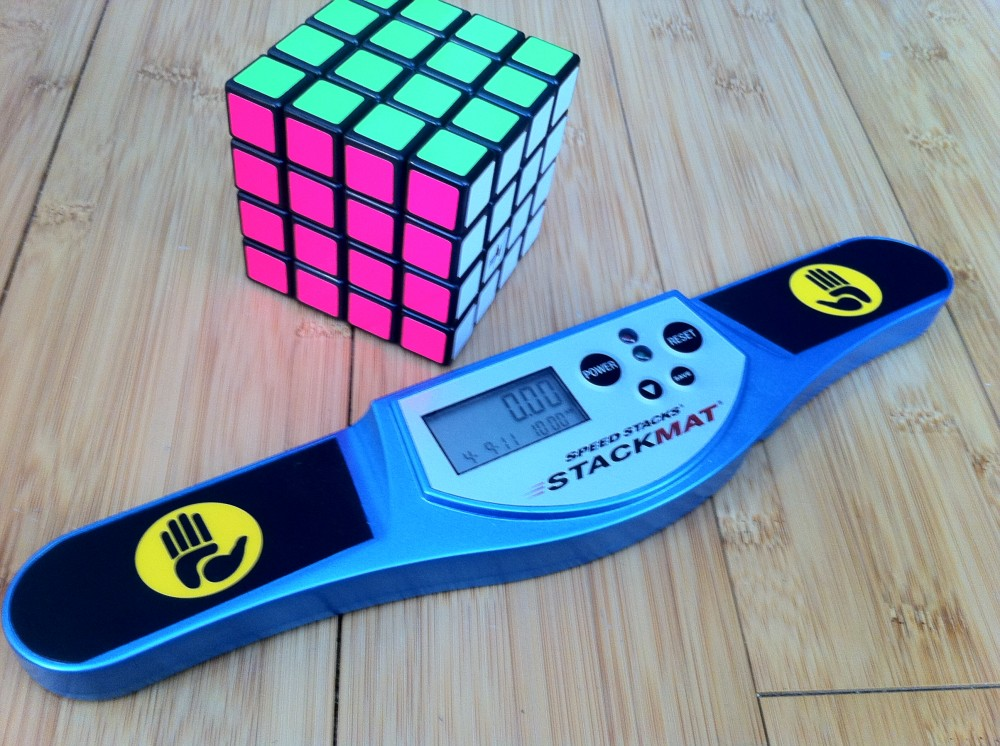
\includegraphics[width=\linewidth,height=0.5\textheight,keepaspectratio]{stackmat.jpg}\\
{\tiny Stackmat, ảnh Protocoldoug, CC0, Wikimedia Commons}

\medskip
\alert{\textbf{Đo từng giây, thấy từng tiến bộ.}}
\end{columns}
\end{frame}

% ================================================================ 2
\begin{frame}{2. Vấn đề và người dùng mục tiêu}
\begin{columns}[T]
\column{0.5\textwidth}
\textbf{Vấn đề}
\begin{itemize}\small
\item Stackmat G5 không tự lưu lịch sử.
\item Nối Stackmat với csTimer bằng dây cáp hay gặp trục trặc.
\item Muốn thấy tiến bộ, người chơi phải tự nhập và tự tính Ao5, Ao12, Ao100.
\end{itemize}
\textbf{Haitay}: mỗi lượt solve tự đi tới biểu đồ, không cần nhập tay.
\column{0.47\textwidth}
\small
\begin{tabular}{L{2.5cm} L{3.0cm}}
\toprule
\hrow \hc{Người dùng} & \hc{Cần gì} \\
\midrule
\srow Người chơi tự luyện tại bàn & Ghi mọi lượt, thấy xu hướng qua nhiều tuần \\
Nhiều người dùng chung thiết bị & Chuyển user, dữ liệu tách riêng \\
\srow Nhiều người chung máy tính & PIN tùy chọn trên máy tính \\
\bottomrule
\end{tabular}

\smallskip
{\footnotesize Haitay là timer luyện tập, bổ trợ cho timer thi đấu.}
\end{columns}
\end{frame}

% ================================================================ 3
\begin{frame}{3. Yêu cầu chức năng: 12 use case}
\centering
\begin{tikzpicture}[
    scale=0.8, transform shape,
    font=\scriptsize,
    uc/.style={draw=haitayblue, fill=haitayblue!8, ellipse, minimum width=3.9cm, minimum height=0.62cm, inner sep=1pt},
    sys/.style={draw=haitayblue, thick, rounded corners=4pt},
    lnk/.style={black!55},
    inc/.style={-{Stealth[length=1.6mm]}, dashed, black!60},
    actor/.pic={\draw[thick] (0,0.62) circle (0.14); \draw[thick] (0,0.48)--(0,0.12) (-0.22,0.36)--(0.22,0.36) (0,0.12)--(-0.17,-0.16) (0,0.12)--(0.17,-0.16);}
]
    \draw[sys] (1.2,0.55) rectangle (6.4,-6.65);
    \node[font=\footnotesize\bfseries, text=haitayblue] at (3.8,0.25) {Thiết bị Haitay};
    \foreach \i/\t in {1/{UC01 Bấm giờ lượt solve}, 2/{UC02 Đánh dấu OK, +2, DNF}, 3/{UC03 Xem thống kê nhanh}, 4/{UC04 Xem, xóa, sửa lượt solve}, 5/{UC05 Mở session mới}, 6/{UC06 Đồng bộ dữ liệu}, 7/{UC07 Chuyển người dùng}} {
        \node[uc] (d\i) at (3.8,-0.88*\i+0.15) {\t};
    }
    \draw[sys] (8.7,0.55) rectangle (13.9,-4.9);
    \node[font=\footnotesize\bfseries, text=haitayblue] at (11.3,0.25) {Phần mềm máy tính};
    \foreach \i/\t in {8/{UC08 Quản lý người dùng}, 9/{UC09 Gắn session với người dùng}, 10/{UC10 Xem dashboard xu hướng}, 11/{UC11 Đăng nhập bằng PIN}, 12/{UC12 Sao lưu, khôi phục}} {
        \node[uc] (p\i) at (11.3,-0.88*\i+7.19) {\t};
    }
    \pic at (0,-3.1) {actor}; \node[align=center] at (0,-3.6) {Người\\chơi};
    \pic at (7.55,-5.6) {actor}; \node[align=center] at (7.55,-6.1) {Dịch vụ\\đồng bộ};
    \pic at (15.0,-2.2) {actor}; \node[align=center] at (15.0,-2.7) {Người dùng\\máy tính};
    \foreach \i in {1,...,7} { \draw[lnk] (0.3,-2.75) -- (d\i.west); }
    \draw[lnk] (7.35,-5.3) -- (d6.east); \draw[lnk] (7.35,-5.3) -- (d7.east);
    \foreach \i in {8,...,12} { \draw[lnk] (14.75,-1.9) -- (p\i.east); }
    \draw[inc] (d1.south east) to[bend left=40] node[right, font=\tiny]{«include»} (d2.north east);
    \draw[inc] (d7.north east) to[bend right=40] node[right, font=\tiny]{«include»} (d6.south east);
\end{tikzpicture}
\end{frame}

% ================================================================ 3b
\begin{frame}{3. Yêu cầu phi chức năng đo được}
\footnotesize
\begin{columns}[T]
\column{0.49\textwidth}
\begin{tabular}{L{0.75cm} L{4.95cm}}
\toprule
\hrow \hc{Mã} & \hc{Chỉ tiêu} \\
\midrule
\srow N1 & Mốc giờ có độ phân giải dưới 1~ms \\
N2 & Trễ phát hiện chạm 2 đến 10~ms; sai lệch solve trong $\pm 10$~ms \\
\srow N3* & Chạm hai tay dưới 1,5~s không làm đồng hồ sẵn sàng \\
N4 & 0 bản ghi đã chốt bị mất qua 100 lần cắt điện \\
\srow N5 & 0 mất, 0 trùng khi rơi kết nối Bluetooth \\
N6 & Trên 100 lượt, thiết kế 512 lượt chưa đồng bộ \\
\bottomrule
\end{tabular}
\column{0.49\textwidth}
\begin{tabular}{L{0.75cm} L{4.95cm}}
\toprule
\hrow \hc{Mã} & \hc{Chỉ tiêu} \\
\midrule
\srow N7* & Đồng bộ 512 bản ghi dưới 10~s \\
N8* & Màn hình 10 lần mỗi giây, đọc được ở 60~cm \\
\srow N9* & Chạy liên tục 24 giờ không khởi động lại \\
N10 & Nguồn USB-C 5~V; pin CR2032 chỉ nuôi đồng hồ thực \\
\srow N11* & Thân một thanh; pad còn nhạy sau 10.000 lần chạm \\
N12* & Module firmware kiểm thử riêng được \\
\bottomrule
\end{tabular}
\end{columns}

\smallskip
Mỗi chỉ tiêu có cách kiểm chứng: máy phân tích logic, relay cắt nguồn, ngắt Bluetooth 20 đến 50 lần.\\
* Ngưỡng do nhóm đề xuất, chờ thống nhất.
\end{frame}

% ================================================================ 4
\begin{frame}{4. Kiến trúc bốn lớp và giao thức từng chặng}
\centering
\resizebox{\linewidth}{!}{%
\begin{tikzpicture}[
    font=\footnotesize,
    own/.style={draw=haitayblue, fill=haitayblue!8, rounded corners=3pt, minimum height=0.85cm, text width=3.3cm, align=center},
    ext/.style={draw=black!45, fill=black!5, rounded corners=3pt, minimum height=0.85cm, text width=2.5cm, align=center},
    lay/.style={font=\footnotesize\bfseries, text=haitayblue, anchor=west, text width=2.5cm, align=left},
    arr/.style={-{Stealth[length=2mm]}, thick, haitayblue},
    lbl/.style={font=\scriptsize, anchor=east, align=right}
]
    \node[lay] at (-0.4,0)    {Thiết bị\\\scriptsize\mdseries lớp cảm nhận};
    \node[lay] at (-0.4,-1.8) {Gateway\\\scriptsize\mdseries lớp mạng};
    \node[lay] at (-0.4,-3.6) {Server\\\scriptsize\mdseries lớp trung gian};
    \node[lay] at (-0.4,-5.4) {Ứng dụng\\\scriptsize\mdseries lớp ứng dụng};
    \node[ext] (pad) at (3.6,0)  {\textbf{Hai pad lá đồng}\\cảm biến chạm};
    \node[own] (mcu) at (8.0,0)  {\textbf{ESP32-S3}\\đo giờ, FRAM, DS3231};
    \node[own] (br)  at (8.0,-1.8) {\textbf{Bridge BLE}\\Python, bleak};
    \node[own] (api) at (8.0,-3.6) {\textbf{Ingest và API}\\Python, FastAPI};
    \node[ext] (db)  at (11.9,-3.6) {\textbf{SQLite}\\một tệp cục bộ};
    \node[own] (ui)  at (8.0,-5.4) {\textbf{Dashboard web}\\Chart.js};
    \draw[arr] (pad) -- node[above, font=\scriptsize]{điện dung} (mcu);
    \draw[arr, <->] (mcu) -- node[lbl, xshift=-10pt]{\textbf{Bluetooth LE}, GATT:\\notify bản ghi, write lệnh} (br);
    \draw[arr, <->] (br)  -- node[lbl, xshift=-10pt]{\textbf{HTTP/REST}, JSON,\\127.0.0.1} (api);
    \draw[arr, <->] (api) -- node[above=1pt, font=\scriptsize]{SQL} (db);
    \draw[arr, <->] (api) -- node[lbl, xshift=-10pt]{\textbf{HTTP/REST}\\và \textbf{SSE}} (ui);
    \begin{scope}[on background layer]
        \node[draw=haitayblue, dashed, rounded corners=6pt, fit=(br)(api)(db)(ui), inner sep=6pt,
              label={[font=\scriptsize\itshape, text=haitayblue]south east:Máy tính của người chơi}] {};
    \end{scope}
\end{tikzpicture}}

\smallskip
{\footnotesize Nền xanh: nhóm tự xây dựng. Nền xám: dùng lại của bên thứ ba.}
\end{frame}

% ================================================================ 4b
\begin{frame}{4. Luồng đồng bộ: không mất, không trùng}
\centering
\begin{tikzpicture}[
    font=\footnotesize,
    blk/.style={draw=haitayblue, fill=haitayblue!8, rounded corners=3pt, minimum width=2.0cm, minimum height=0.8cm, align=center, font=\footnotesize\bfseries},
    fwd/.style={-{Stealth[length=2mm]}, thick, haitayblue},
    bck/.style={-{Stealth[length=2mm]}, thick, haitayorange, dashed},
    m/.style={font=\scriptsize, align=center}
]
    \node[blk] (d) at (0,0)    {Thiết bị\\[-0.2em]\scriptsize\mdseries FRAM};
    \node[blk] (b) at (3.9,0)  {Bridge BLE};
    \node[blk] (a) at (7.8,0)  {Ingest};
    \node[blk] (s) at (11.3,0) {SQLite};
    \draw[fwd] ([yshift=4pt]d.east) -- node[above, m]{notify LOG\\11 bản ghi} ([yshift=4pt]b.west);
    \draw[fwd] ([yshift=4pt]b.east) -- node[above, m]{POST \texttt{/ingest}} ([yshift=4pt]a.west);
    \draw[fwd] ([yshift=4pt]a.east) -- node[above, m]{COMMIT} ([yshift=4pt]s.west);
    \draw[bck] ([yshift=-4pt]a.west) -- node[below, m]{\texttt{last\_seq}} ([yshift=-4pt]b.east);
    \draw[bck] ([yshift=-4pt]b.west) -- node[below, m]{\texttt{ACK(seq)}\\sau COMMIT} ([yshift=-4pt]d.east);
\end{tikzpicture}

\bigskip
\raggedright\small
\begin{tabular}{L{4.3cm} L{7.0cm}}
\toprule
\hrow \hc{Bất biến} & \hc{Cơ chế duy nhất bảo đảm} \\
\midrule
\srow Chưa ACK thì không bị ghi đè & Chỉ ghi vào ô có seq $\le$ \texttt{last\_ack}; đầy thì từ chối lượt mới \\
Chỉ ACK phần đã nằm trên đĩa & \texttt{ACK} gửi sau khi giao dịch SQLite COMMIT \\
\srow Gửi lại không tạo bản sao & Khóa chính \texttt{(device\_id, seq)} \\
\bottomrule
\end{tabular}
\end{frame}

% ================================================================ 5
\begin{frame}{5. Thiết bị, chi phí và lợi ích}
\begin{columns}[T]
\column{0.64\textwidth}
\footnotesize
\begin{tabular}{L{4.5cm} C{0.4cm} R{1.5cm}}
\toprule
\hrow \hc{Linh kiện} & \hc{SL} & \hc{Đơn giá (đ)} \\
\midrule
\srow Bo ESP32-S3 (1 dự phòng) & 2 & 295.000 \\
TFT 1,54 inch ST7789, SPI & 1 & 85.000 \\
\srow FRAM FM24CL64B, 8~KB & 2 & 153.000* \\
DS3231 kèm pin CR2032 & 1 & 44.000 \\
\srow MPR121 (dự phòng cảm biến) & 1 & 25.000 \\
Lá đồng, dây, ba nút nhấn & 1 & 130.000* \\
\srow Vỏ in 3D, hai lần in & 2 & 96.000 \\
\midrule
\textbf{Tổng (đã gồm số lượng)} & & \textbf{1.372.000} \\
\bottomrule
\end{tabular}

{\tiny Giá quan sát tháng 10/2026, chưa gồm vận chuyển; * là ước lượng.}
\column{0.33\textwidth}
\textbf{Lợi ích dự kiến}
\begin{itemize}\footnotesize
\item Một bộ hoàn chỉnh khoảng 803.000 đồng; Stackmat G5 giá 0,9 đến 1,0 triệu.
\item Không nhập tay từ lượt solve tới biểu đồ.
\item Dữ liệu ở lại máy người chơi, không phí dịch vụ.
\end{itemize}
\end{columns}
\end{frame}

% ================================================================ 6
\begin{frame}{6. Lựa chọn công nghệ và lý do}
\footnotesize
\setlength{\tabcolsep}{4pt}
\begin{tabular}{L{2.1cm} L{2.2cm} L{2.2cm} L{5.8cm}}
\toprule
\hrow \hc{Hạng mục} & \hc{Chọn} & \hc{Không chọn} & \hc{Lý do} \\
\midrule
\srow Truyền thông & Bluetooth LE & Wi-Fi, Zigbee & Cách vài mét, vài KB mỗi buổi; USB-C dự phòng \\
Vi điều khiển & ESP32-S3 N8 & Pico 2 W; STM32WB55 dự phòng & Chạm và BLE có sẵn; hệ sinh thái trưởng thành \\
\srow Lưu trên thiết bị & FRAM & EEPROM; flash dự phòng & Ghi tức thì, $10^{14}$ lần ghi, chịu rút cáp \\
Gateway tới server & HTTP/REST & MQTT & PUBACK chỉ báo broker đã nhận, chưa báo CSDL đã lưu \\
\srow Cơ sở dữ liệu & SQLite & InfluxDB & Vài MB, cần quan hệ và khóa chống trùng \\
Backend & Python: bleak, FastAPI & Web Bluetooth & Chạy nền, tự nối lại; Web Bluetooth phải bấm mỗi lần \\
\srow Web & Chart.js, SSE & WebSocket & Chỉ cần đẩy một chiều, SSE tự nối lại \\
\bottomrule
\end{tabular}
\end{frame}

% ================================================================ 7
\begin{frame}{7. Tiến độ: luồng dữ liệu đầu cuối}
\small
Linh kiện chưa về đủ, nên nhóm chạy cả luồng bằng \textbf{mô phỏng Python}. Logic bản ghi, CRC, đồng bộ và lược đồ là mã thật.

\medskip
\centering
\begin{tikzpicture}[
    font=\scriptsize,
    done/.style={draw=haitaygreen, fill=haitaygreen!10, rounded corners=3pt, text width=2.65cm, minimum height=1.5cm, align=center},
    todo/.style={draw=black!40, fill=black!5, rounded corners=3pt, text width=2.65cm, minimum height=0.9cm, align=center},
    hd/.style={font=\footnotesize\bfseries, text=haitayblue},
    arr/.style={-{Stealth[length=2mm]}, thick, haitayblue}
]
    \foreach \px/\nm/\hdr/\txt in {0/s/Cảm biến/{Tín hiệu hai pad 1~kHz, trễ 2 đến 10~ms; máy trạng thái, FRAM ảo},
                             3.4/p/Giao thức/{Khung LOG 11 bản ghi, \texttt{ACK}, \texttt{SET\_TIME} qua BLE ảo},
                             6.8/d/Cơ sở dữ liệu/{SQLite, khóa \texttt{(device\_id, seq)}, ACK sau COMMIT},
                             10.2/u/Giao diện/{Truy vấn Ao5, Ao12, Ao100; biểu đồ xuất tệp tĩnh}} {
        \node[hd] at (\px,1.15) {\hdr};
        \node[done] (\nm) at (\px,0) {\txt};
    }
    \foreach \a/\b in {s/p, p/d, d/u} { \draw[arr] (\a) -- (\b); }
    \foreach \px/\txt in {0/{Chưa có: ESP32-S3 và pad thật}, 3.4/{Chưa có: GATT NimBLE, bleak}, 6.8/{Chưa có: dịch vụ FastAPI}, 10.2/{Chưa có: Chart.js và SSE}} {
        \node[todo] at (\px,-1.45) {\txt};
    }
\end{tikzpicture}

\medskip
\raggedright
Khung xanh: đã chạy trong mô phỏng. Khung xám: việc chuyển sang phần cứng và web.
\end{frame}

% ================================================================ 7b
\begin{frame}{7. Kết quả mô phỏng: 17/17 phép kiểm tra đạt}
\footnotesize
\begin{tabular}{L{0.7cm} L{4.8cm} L{7.0cm}}
\toprule
\hrow \hc{Mã} & \hc{Kịch bản bất lợi} & \hc{Kết quả đo được} \\
\midrule
\srow T1 & 400 lượt, trễ cảm biến 2 đến 10~ms & Sai lệch TB $-0{,}01$~ms, SD 3,26~ms, trong $[-7, 7]$~ms \\
S2 & Rơi BLE sau khung 7, mất một ACK & 3 lần kết nối, 11 bản ghi gửi lại bị loại trùng \\
\srow S3 & 100 lần cắt điện giữa lúc ghi & 0 bản ghi đã chốt bị mất \\
S4 & Một khung bị lật một byte & Bị từ chối, lần kết nối sau gửi lại đủ \\
\srow S5 & 512 lượt chưa đồng bộ & Lượt 513 bị từ chối tới khi đồng bộ \\
S7 & Chuyển người dùng A sang B & WIPE bị từ chối khi chưa ACK; A 30 lượt, B 12 lượt \\
\bottomrule
\end{tabular}

\medskip
\small Lần chạy 13/11/2026, hạt giống cố định: \texttt{python -I code/sim/run\_scenarios.py}
\end{frame}

% ================================================================ 7c
\begin{frame}{7. Kết quả mô phỏng: đo giờ và dữ liệu mẫu}
\begin{columns}[T]
\column{0.5\textwidth}
\centering
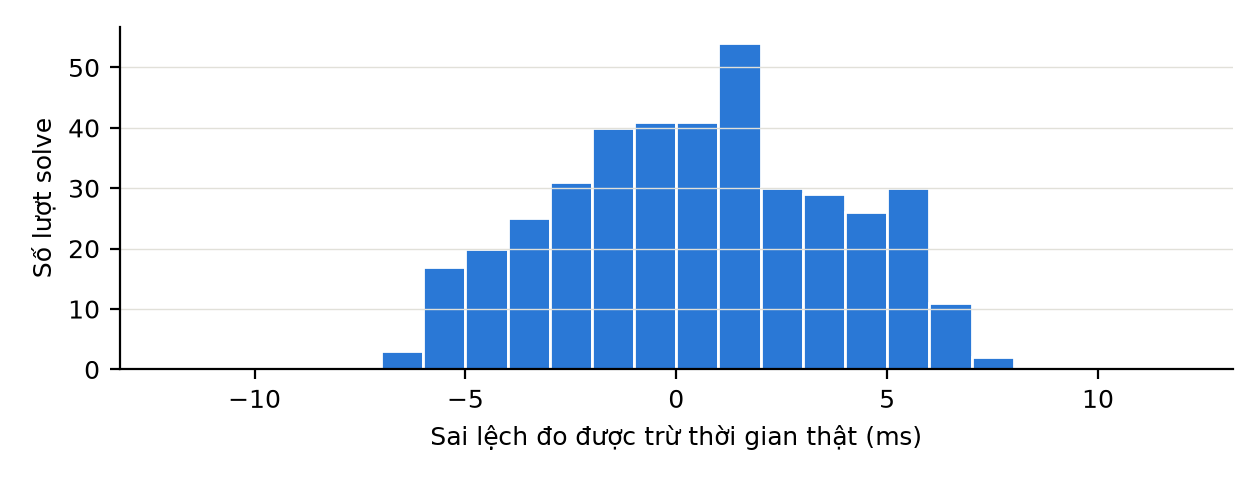
\includegraphics[width=\linewidth,height=0.62\textheight,keepaspectratio]{sim_timing.png}\\
\footnotesize Firmware không cộng thêm sai số ngoài độ trễ cảm biến
\column{0.5\textwidth}
\centering
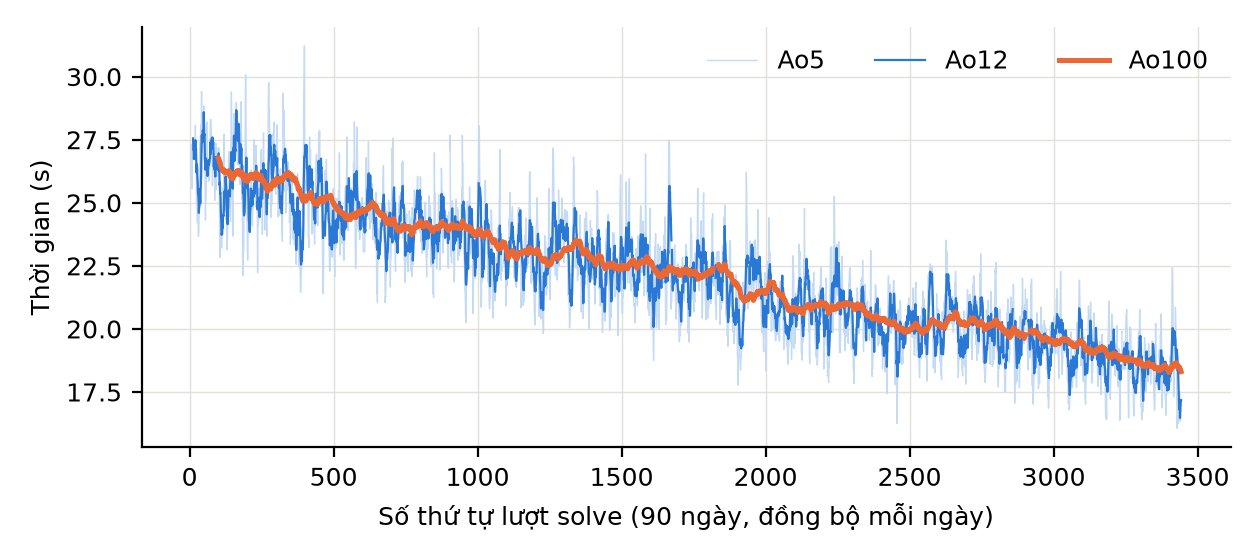
\includegraphics[width=\linewidth,height=0.62\textheight,keepaspectratio]{sim_rolling.png}\\
\footnotesize 90 ngày, 3.443 lượt đồng bộ qua giao thức thật, truy vấn từ SQLite
\end{columns}
\end{frame}

% ================================================================ 7d
\begin{frame}{7. Mô phỏng Wokwi trên ESP32-S3}
\begin{columns}[T]
\column{0.55\textwidth}
\centering
\begin{tikzpicture}
    \node[draw=red!75!black, dashed, rounded corners=4pt, minimum width=6.8cm, minimum height=4.2cm, align=center, font=\small]
        {\cbs{cần bổ sung: ảnh chạy Wokwi}\\[0.4em]\footnotesize thay bằng \texttt{wokwi\_*.png} khi có};
\end{tikzpicture}
\column{0.42\textwidth}
\small
\begin{itemize}
\item Hai pad thay bằng nút nhấn, vì Wokwi không mô phỏng cảm ứng điện dung và BLE.
\item Mỗi lượt đã chốt in ra cổng nối tiếp một dòng \texttt{REC}.
\item \texttt{wokwi\_ingest.py} nạp các dòng đó vào SQLite.
\end{itemize}
\end{columns}
\end{frame}

% ================================================================ 8
\begin{frame}{8. Phân công, kho mã và khó khăn}
\begin{columns}[T]
\column{0.55\textwidth}
\footnotesize
\begin{tabular}{L{2.6cm} L{4.0cm}}
\toprule
\hrow \hc{Thành viên} & \hc{Phụ trách} \\
\midrule
\srow Phạm Gia Hưng & Điều phối, tích hợp, mô phỏng, báo cáo \\
Đỗ Trường Giang & Thiết bị: lắp mạch, firmware, đo trễ \\
\srow Dương Thanh Minh & Backend: bridge BLE, ingest, SQLite \\
Nguyễn Anh Bảo & Dashboard web, kịch bản demo \\
\bottomrule
\end{tabular}

\smallskip
Phân công đề xuất: \cbs{cần bổ sung: nhóm xác nhận}\\
Kho mã: \cbs{cần bổ sung: link repository}
\column{0.42\textwidth}
\textbf{Khó khăn và rủi ro lớn nhất}
\begin{itemize}\footnotesize
\item FRAM FM24CL64B không bán trong nước, giao 1 đến 3 tuần.
\item Bluetooth LE dễ trễ tiến độ; giao thức đã chốt và kiểm thử trước.
\item Đo độ trễ tuyệt đối cần thiết bị tham chiếu.
\item Cảm biến chạm có thể kích hoạt sai khi tay ẩm hoặc gần bộ sạc.
\end{itemize}
\end{columns}
\end{frame}

\begin{frame}[standout]
Cảm ơn thầy và các bạn\\[0.4em]
\normalsize Đo từng giây, thấy từng tiến bộ.
\end{frame}

\end{document}
